\chapter{Results}

\section{Steering Clear Reproduction}

\begin{figure}
    \centering
    \captionsetup{width=\textwidth}
    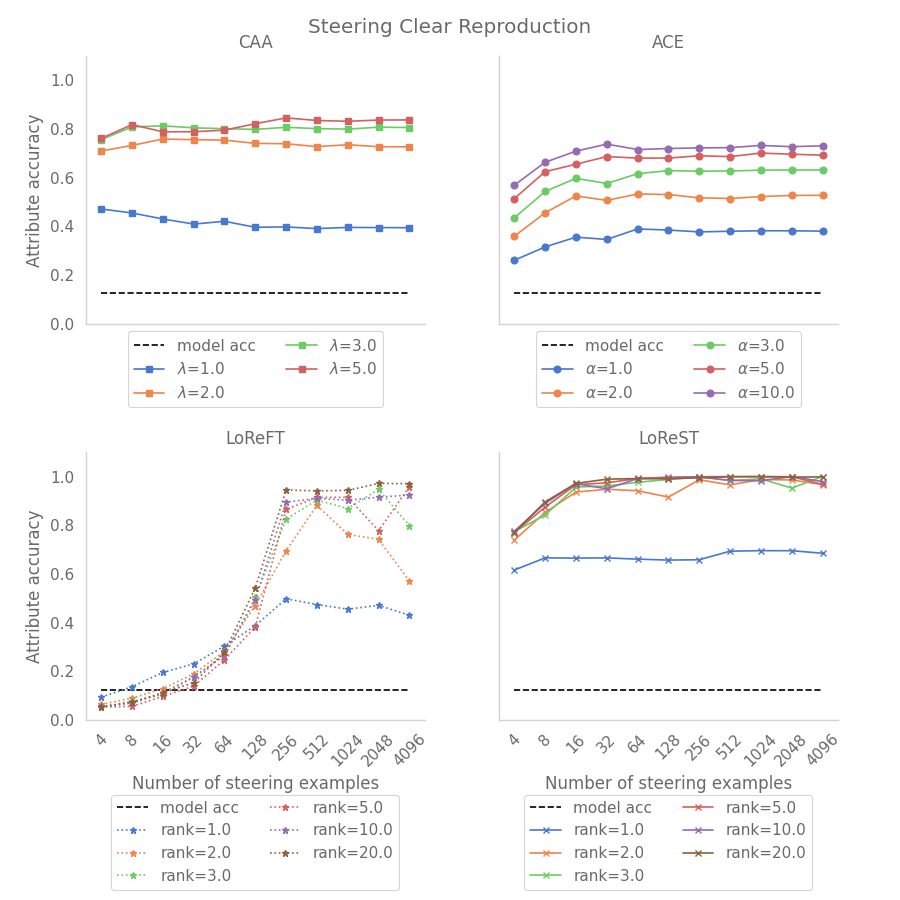
\includegraphics[width=\textwidth]{figures/steering_clear.png}
    \caption{
        Reproduction of Figure 1 (top-left) in \citet{steering-clear}.
        Instead of overlaying all the data in a single plot the for methods are separated.
        ACE \citep{ace} is introduced and MiMiC \citep{mimic} is removed.
        Though the metric is different, focusing on the steered attribute rather than all attributes, the same trends are presents.
        The model accuracy is changed to reflect the accuracy of the model without steering rather than the model accuracy on the target input.
    }
    \label{fig:steering-clear}
\end{figure}

Following the experiment described in \Sref{sec:steering-clear} the results of \cite{steering-clear} are reproduced in \Fref{fig:steering-clear}.
There are a few changes from Figure 1 in \cite{steering-clear}, primarily the steering metric focuses on the steered attribute rather than entire output label.
Furthermore, affine concept editting (ACE) \citep{ace} is added and minimally modified counterfactuals (MiMiC) \citep{mimic} is removed.
A full discussion of the different metric and why this was used is presented in \Sref{app:steering-clear}.

\Fref{fig:steering-clear} only represents the upper-left plot in \cite{steering-clear} Figure 1.
This reproduction aims to verify the method used in \cite{steering-clear} and the results achieved as a stepping stone towards carrying out a similar analysis for large language models (LLMs).

The figure clearly shows a difference between the linear/affine methods of contrastive activation addition (CAA) \citep{caa} \& ACE and the low-rank methods of low-rank representation finetuning (LoReFT) \citep{reft} \& low-rank representation steering (LoReST) \citep{steering-clear}.
In the limit of more examples both low-rank methods achieve near 100\% success rate in steering the target attribute to the target value.
In comparison the affine methods reach an asymptote which does not increase with more training examples.
Importantly, in the low training example setting both LoReFT performs worse than both CAA and ACE.
In fact, it performs worse than the model without steering.
This is due to the requirement to train parameters which both affine approaches lack.
However, the addition of parameters allows the method to perform better as more examples are presented.
This feature of improvement with more examples is shared with LoReST.

Across the methods there is a critical hyperparameter above which the methods perform comparably.
In the case of CAA (in this environment) this appears to be $\lambda=2$.
For LoReFT the threshold rank is likely 3 as 2 decreases in accuracy as more examples are introduced.
Finally with LoReST the rank is clearly 2.
ACE behaves differently due to it's design (detailed in \Sref{sec:ace}) where the parameters relate to the strength of the behaviour more directly.
This is visible in \Fref{fig:steering-clear} as clear bands as the hyperparameter increases; in comparison to the other plots where after a threshold hyperparameter value the adaptors behave similarly.

Similar to the findings of \citet{steering-clear} LoReFT plateaus after 256 examples which coincides with the dimension of the activation space.
This distinction is not present in the other methods though this is similar to the Figure in \citet{steering-clear}.
A possible explanation for this in the case of the affine methods is they do not learn their own representation.
Instead, with sufficient opposing examples, the difference in steering direction is minimal with more examples.

LoReST in comparison to both LoReFT and the affine examples incorporates both approaches.
This means in the low data regime it likely behaves closer to ACE and CAA, then when enough data is provided that it can encode the concepts sufficiently the accuracy increases.
This is supported by the fact that LoReST achieves $\sim 0.8$ with 4 examples matching CAA, LoReST then continues to increase in accuracy following a similar arc to ACE eventually plateauing at the same values as LoReFT.
This behaviour is matched in \citet{steering-clear}.

Overall, the results suggest that the analysis by \citet{steering-clear} are sound though an exact replication was not achieved.
This also suggests some expectations for the prompt pairs environment (described in \Sref{sec:prompt-pairs}).
In particular
\begin{itemize}[nolistsep]
    \item Affine methods will perform consistently across the number of examples used, though minor variation may occur.
    \item Low rank methods will increase with the number examples eventually plateauing.
    \item LoReST is likely to achieve the best performance.
\end{itemize}

\section{Prompt Pairs}

\begin{figure}
    \centering
    \captionsetup{width=\textwidth}
    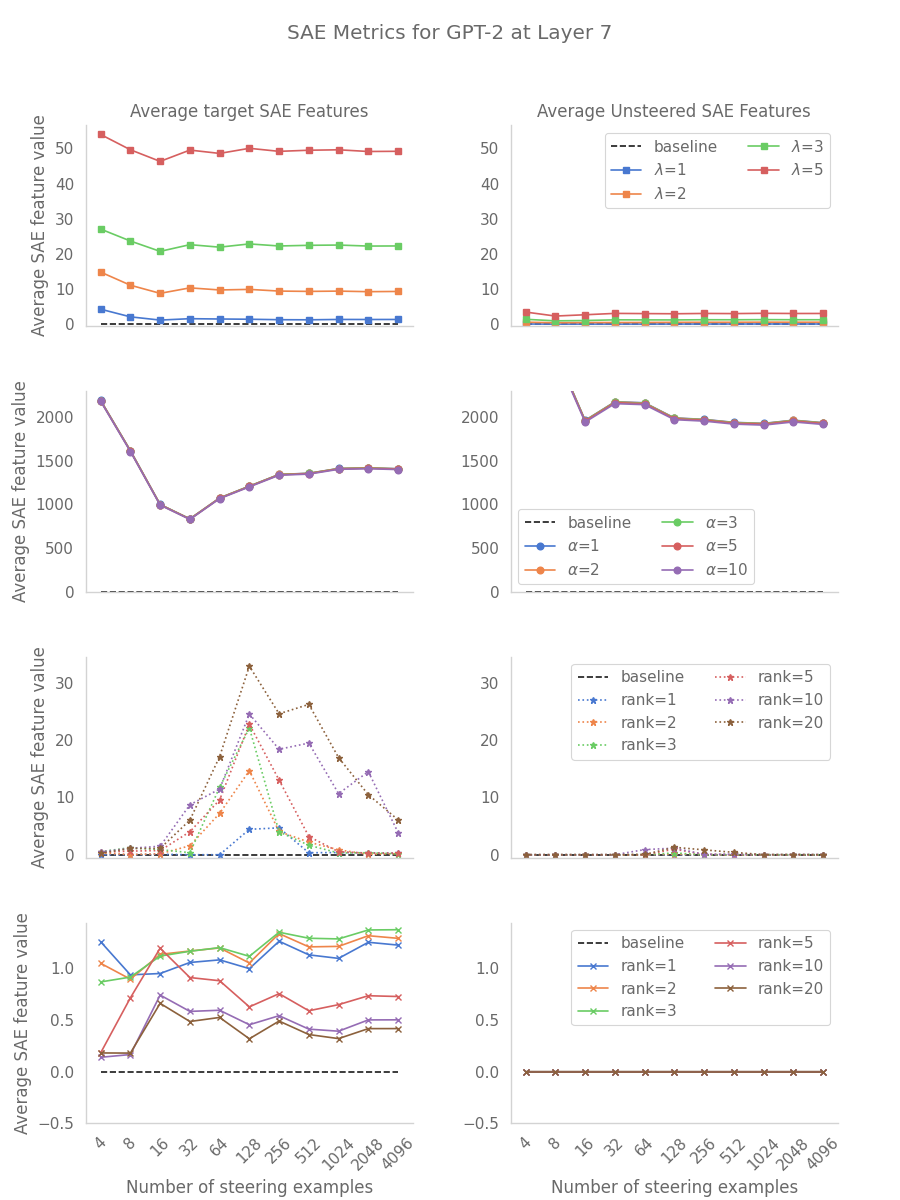
\includegraphics[width=\textwidth]{figures/gpt2_7_sae.png}
    \caption{
        The average activation of SAE features for the set of target SAE features and unsteered SAE features.
        From top to bottom the rows represent CAA \citep{caa}, ACE \citep{ace}, LoReFT \citep{reft} and LoReST \citep{steering-clear}.
        The same range of examples is used across all adaptors.
        The exact SAE feature values are only important in the unsteered case, where they should be 0, or as a comparison within the model parameters.
    \Sref{sec:prompt-pairs} describes how these metrics are calculated.}
    \label{fig:gpt-pp-sae}
\end{figure}

\begin{figure}
    \centering
    \captionsetup{width=.9\textwidth}
    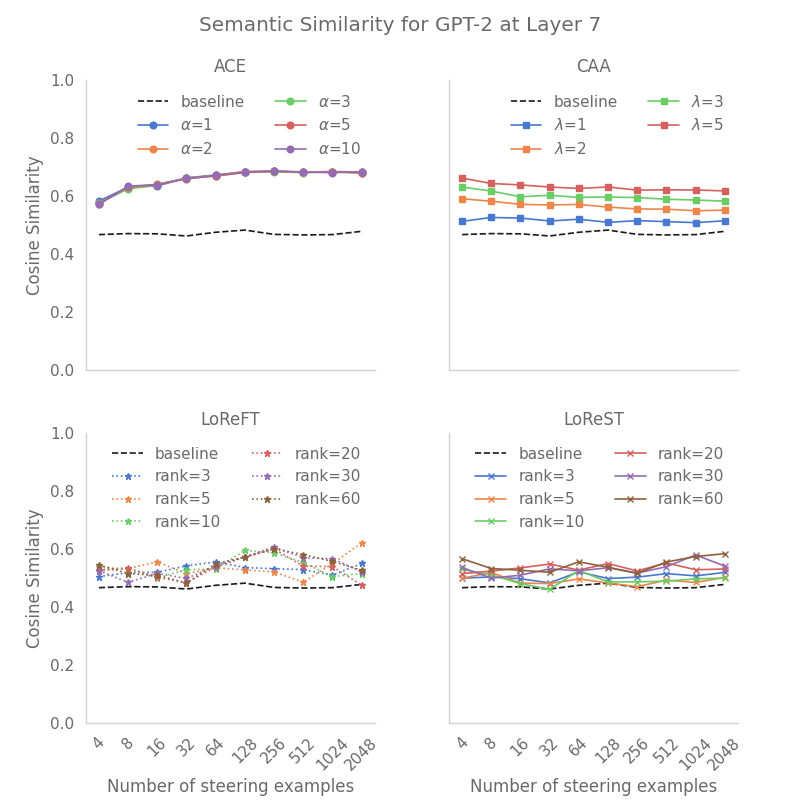
\includegraphics[width=\textwidth]{figures/gpt2_7_similarity.png}
    \caption{
        The cosine similarity of distilbert \citep{distilbert} word embeddings for the generated token.
        The number of steering examples is the same as \Fref{fig:steering-clear} and the cosine similarity is shared across charts.
        Note that the y axis has been cropped to highlight the difference between models though the change is slight.
    }
    \label{fig:gpt-pp-sim}
\end{figure}

